\documentclass[11pt,a4paper]{article}
\usepackage[utf8]{inputenc}
\usepackage[spanish]{babel}	%Idioma
\usepackage{amsmath}
\usepackage{amsfonts}
\usepackage{amssymb}
\usepackage{graphicx} 	%Añadir imágenes
\usepackage{geometry}	%Ajustar márgenes
\usepackage[export]{adjustbox}[2011/08/13]
\usepackage{float}
\restylefloat{table}
\usepackage[hidelinks]{hyperref}
\usepackage{titling}
\graphicspath{{/home/nazaret/Escritorio/LaTEX}}
%\usepackage{minted}
\usepackage{multirow}
\usepackage{caption}
\usepackage{multicol}
\usepackage[shortlabels]{enumitem}
\usepackage{array}
\selectlanguage{spanish}

%Opciones de encabezado y pie de página:
\usepackage{fancyhdr}
\pagestyle{fancy}
\lhead{Nazaret Román Guerrero}
\rhead{Redes Multiservicio}
\lfoot{Grado en Ingeniería Informática}
\cfoot{}
\rfoot{\thepage}
\renewcommand{\headrulewidth}{0.4pt}
\renewcommand{\footrulewidth}{0.4pt}

%Opciones de fuente:
\usepackage[utf8]{inputenc}
\usepackage[default]{sourcesanspro}
\usepackage{sourcecodepro}
\usepackage[T1]{fontenc}

\setlength{\parindent}{15pt}
\setlength{\headheight}{15pt}
\setlength{\voffset}{10mm}

% Custom colors
\usepackage{color}
\definecolor{deepblue}{rgb}{0,0,0.5}
\definecolor{deepred}{rgb}{0.6,0,0}
\definecolor{deepgreen}{rgb}{0,0.5,0}

\usepackage{listings}
\lstset{basicstyle=\ttfamily,
  showstringspaces=false,
  commentstyle=\color{red},
  keywordstyle=\color{blue}
}

\begin{document}
\begin{titlepage}

\begin{minipage}{\textwidth}

\centering
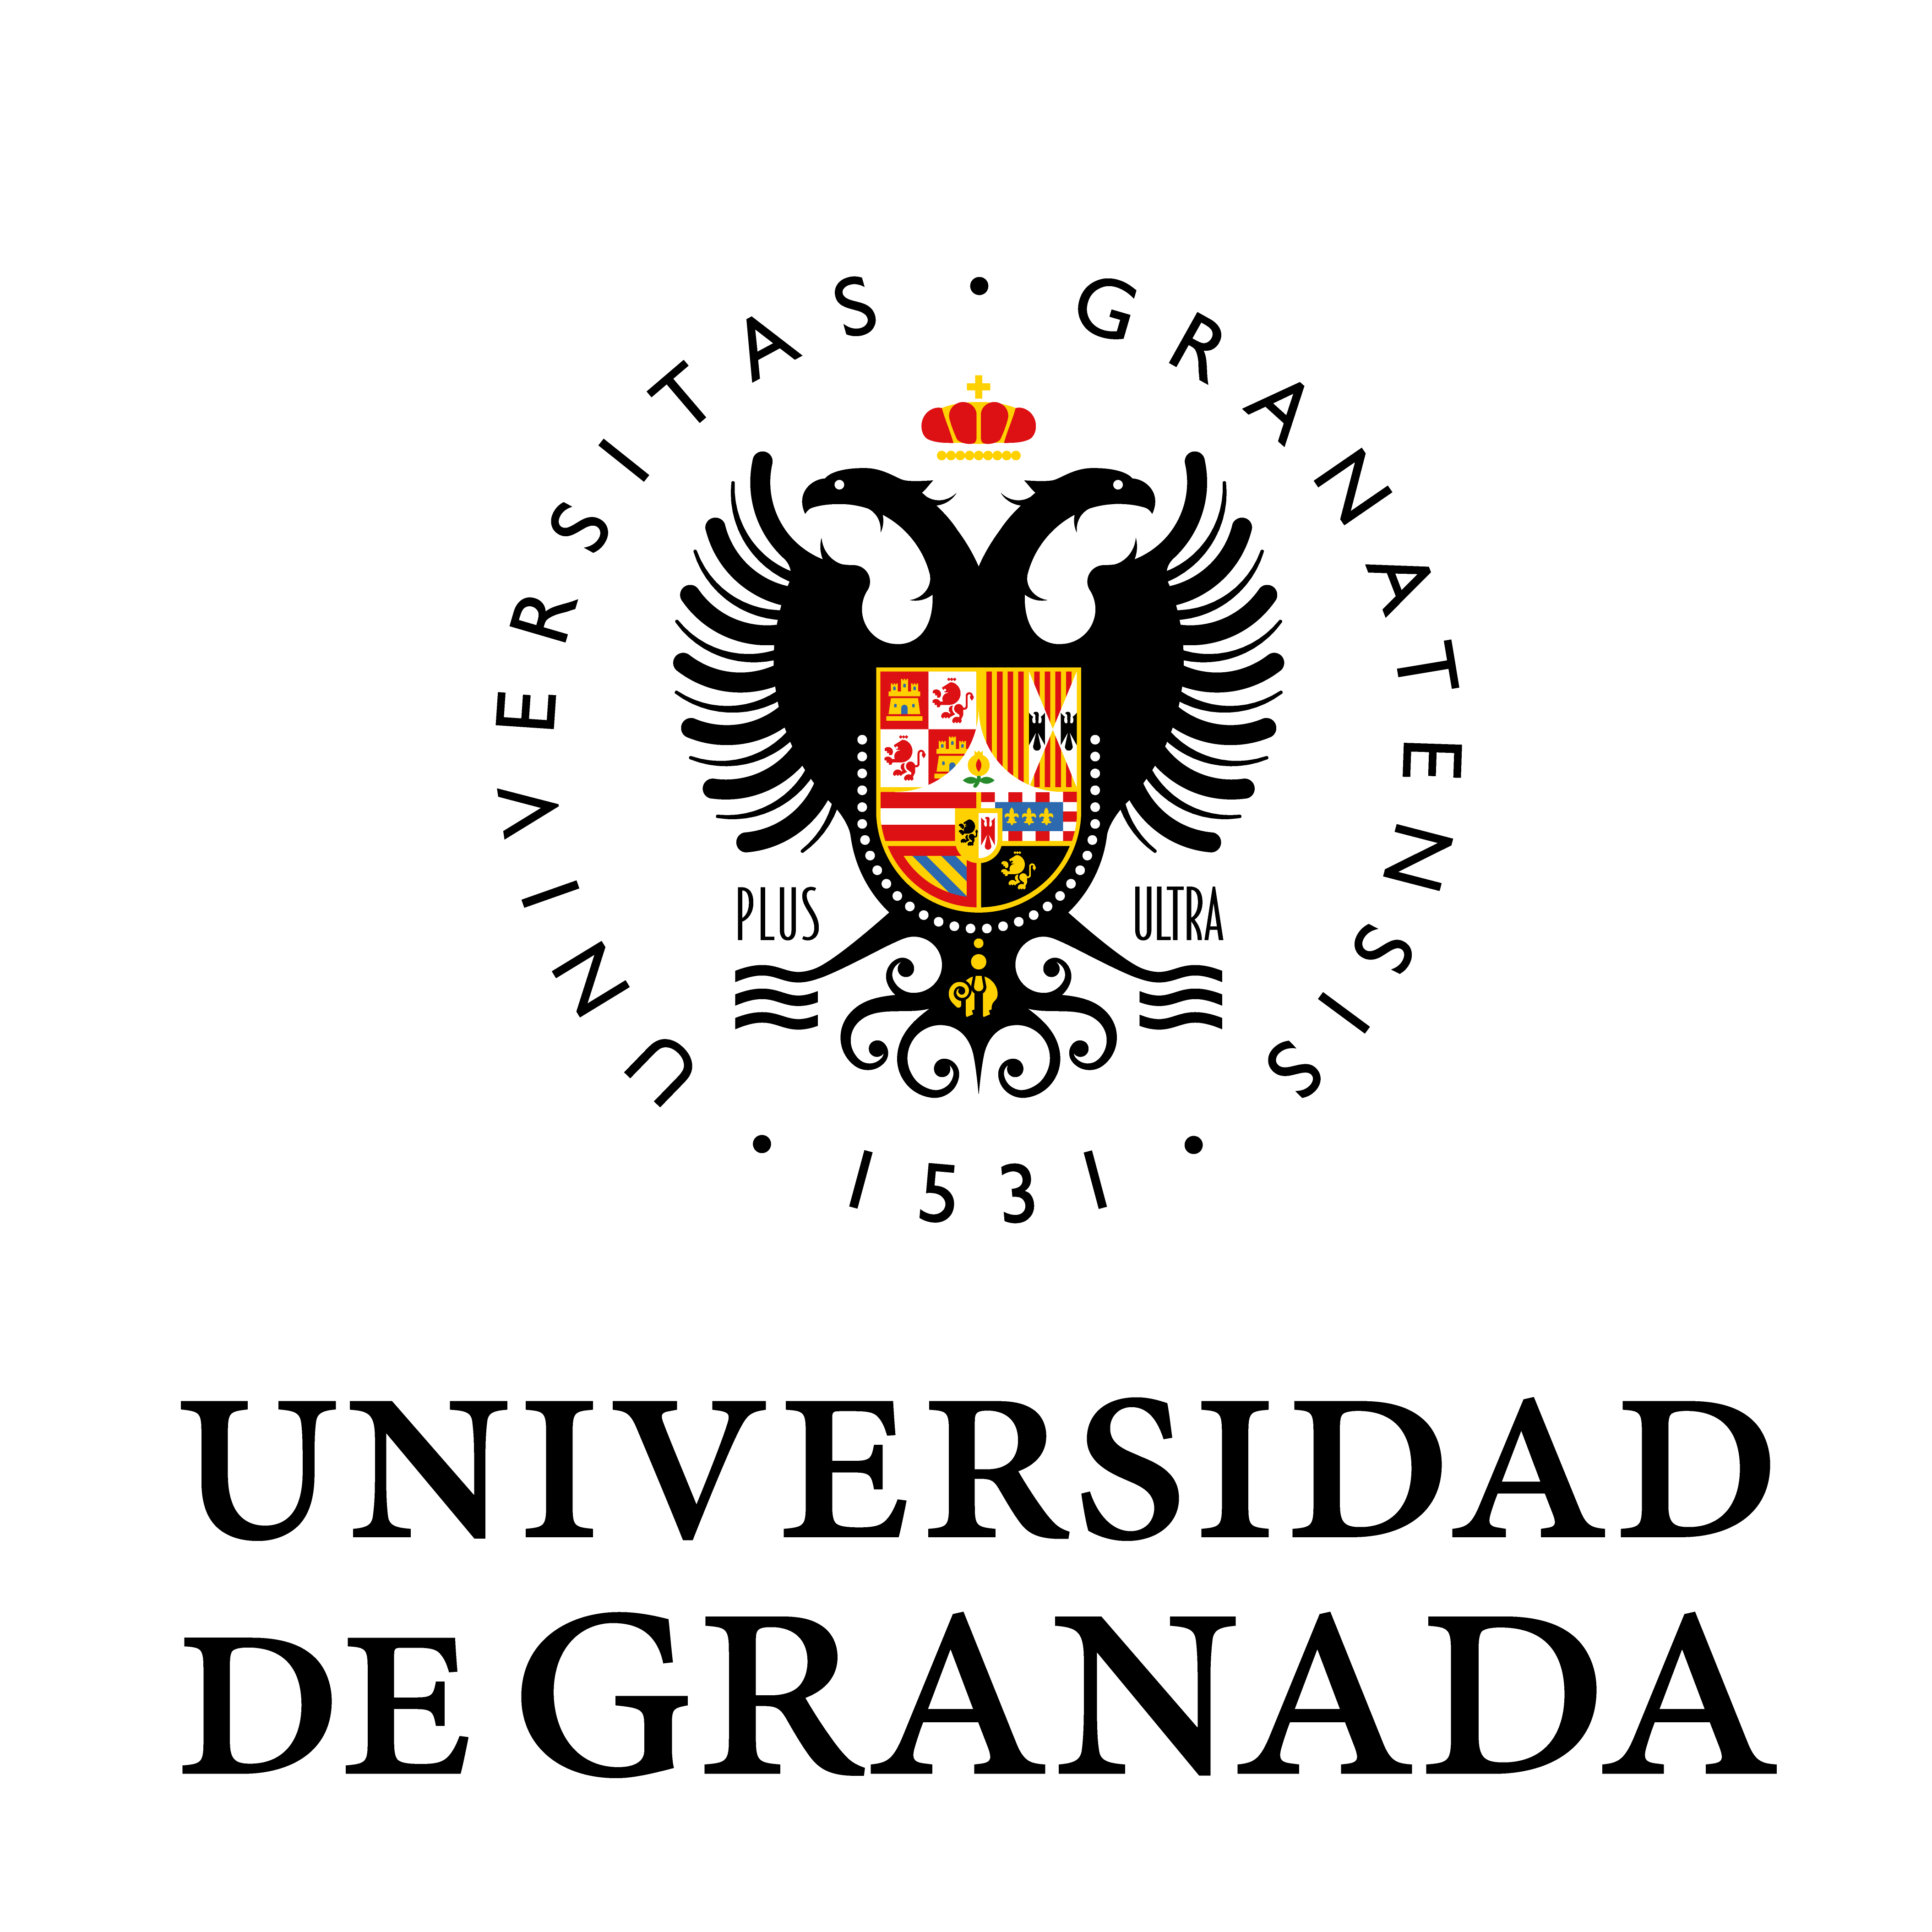
\includegraphics[width=0.5\textwidth]{logo.png}\\

\textsc{\Large asignatura\\[0.2cm]}
\textsc{GRADO EN INGENIERÍA INFORMÁTICA}\\[1cm]

{\Huge\bfseries Práctica 3\\}
\noindent\rule[-1ex]{\textwidth}{3pt}\\[3.5ex]
{\large\bfseries Implementación de un servicio telemático basado en webcam}
\end{minipage}

\vspace{1.5cm}
\begin{minipage}{\textwidth}
\centering

\textbf{Autora}\\ {Nazaret Román Guerrero}\\[2.5ex]

\includegraphics[width=0.3\textwidth]{etsiit.jpeg}\\[0.1cm]
\vspace{1cm}
\textsc{Escuela Técnica Superior de Ingenierías Informática y de Telecomunicación}\\
\vspace{1cm}
\textsc{Curso 2019-2020}
\end{minipage}
\end{titlepage}

\pagenumbering{gobble}
\pagenumbering{arabic}
\tableofcontents
\thispagestyle{empty}

\newpage

\section{Servidor y cliente TCP}

\color{deepgreen}\textbf{Archivos: \texttt{ServidorTCP} y \texttt{ClienteTCP}}.\color{black}\\

Crear el servidor que usa TCP es sencillo. El servidor solo necesita abrir un \textit{socket} o tubería para conectarse con los clientes (\texttt{ServerSocket}) y otro \textit{socket} para aceptar la petición de cada cliente.\\

Cuando un cliente envía una petición, abre la webcam y toma una foto, que envía a través de la tubería al cliente. El servidor está escuchando continuamente peticiones de clientes.\\

Por otro lado, el cliente solo necesita conectarse al mismo puerto que el servidor con un \textit{socket}. Una vez hecho esto, el servidor envía la imagen y el cliente solo debe mostrarla en un frame.

\section{Servidor y cliente UDP}

\color{deepgreen}\textbf{Archivos: \texttt{ServidorUDP} y \texttt{ClienteUDP}}.\color{black}

\subsection{Servidor}

A diferencia del servidor TCP, en el UDP debemos tener más cosas en cuenta.\\

El servidor UDP necesita recibir una petición en forma de datagrama (p. ej. una cadena de texto como en mi caso).  El servidor abre la cámara y toma la foto.\\

Cuando ya la tiene, la descompone en píxeles para calcular el número de datagramas que va a necesitar mandarle al cliente y avisarlo. Los datagramas que he puesto son de 4096 bytes.\\

Una vez enviado al cliente el número de datagramas, el servidor transforma los píxeles a bytes, los mete en un array y los envía en forma de datagrama al cliente mediante un bucle \texttt{for} hasta que ha terminado de enviar la imagen completa. Entre cada envío, el servidor espera 2 segundos.

\subsection{Cliente}

Por otro lado, el cliente envía una petición al servidor para que le envíe la imagen. Cuando ya lo ha hecho, el cliente espera que el servidor le conteste con el número de datagramas a enviar. Cuando ya los sabe, el cliente empieza a recibir todos los datagramas con los bytes de la imagen.\\

Con los datagramas recibidos, reconstruimos la imagen en el cliente y la mostramos en un frame.

\section{Opcional: Servidor TCP concurrente}

\color{deepgreen}\textbf{Archivos: \texttt{SCTCP} y \texttt{ClienteTCP}}.\color{black}\\

Utilizando de base el servidor TCP previo, podemos utilizar hebras para crear el concurrente. La clase tendrá un atributo que se corresponderá con el cliente que va a atender cada instancia de la clase.\\

Cada petición de un cliente crea una hebra que atenderá la petición. Esta hebra abrirá la cámara, tomará la foto, la enviará al cliente y cerrará la cámara para que otra hebra pueda usarla.\\

El cliente es exactamente igual que el cliente TCP sin concurrencia, por lo que no hay ningún archivo con su implementación.

\end{document}